\documentclass[aspectratio=169,10pt]{beamer}

% --------------------------------------------------------------------------
% Theme & colours
% --------------------------------------------------------------------------
\usetheme{default}
\usecolortheme{default}

% BL-1 brand colours
\definecolor{bl1blue}{HTML}{2563EB}
\definecolor{bl1dark}{HTML}{1E293B}
\definecolor{bl1light}{HTML}{F1F5F9}
\definecolor{bl1green}{HTML}{16A34A}
\definecolor{bl1amber}{HTML}{D97706}
\definecolor{bl1red}{HTML}{DC2626}

\setbeamercolor{structure}{fg=bl1blue}
\setbeamercolor{title}{fg=bl1dark}
\setbeamercolor{frametitle}{fg=bl1dark,bg=bl1light}
\setbeamercolor{block title}{fg=white,bg=bl1blue}
\setbeamercolor{block body}{bg=bl1light}
\setbeamercolor{itemize item}{fg=bl1blue}
\setbeamercolor{itemize subitem}{fg=bl1blue!70}
\setbeamertemplate{navigation symbols}{}
\setbeamertemplate{footline}[frame number]

% --------------------------------------------------------------------------
% Packages
% --------------------------------------------------------------------------
\usepackage[T1]{fontenc}
\usepackage{lmodern}
\usepackage{tikz}
\usetikzlibrary{arrows.meta,positioning,shapes.geometric,calc,fit,backgrounds}
\usepackage{listings}
\usepackage{booktabs}
\usepackage{xcolor}
\usepackage{graphicx}

% --------------------------------------------------------------------------
% Listings style (Python-like pseudocode)
% --------------------------------------------------------------------------
\lstdefinestyle{pseudo}{
  basicstyle=\ttfamily\scriptsize,
  keywordstyle=\bfseries\color{bl1blue},
  commentstyle=\itshape\color{gray},
  stringstyle=\color{bl1green},
  showstringspaces=false,
  columns=flexible,
  keepspaces=true,
  morekeywords={for,in,def,return,import,from,class,if,else,while},
  literate={+}{{{\color{bl1dark}+}}}1
           {=}{{{\color{bl1dark}=}}}1
           {*}{{{\color{bl1dark}*}}}1,
  backgroundcolor=\color{bl1light},
  frame=single,
  rulecolor=\color{bl1blue!30},
  framesep=4pt,
  xleftmargin=6pt,
  xrightmargin=6pt,
}
\lstset{style=pseudo}

% --------------------------------------------------------------------------
% Title
% --------------------------------------------------------------------------
\title{\textbf{BL-1}}
\subtitle{GPU-Accelerated In-Silico Cortical Culture Simulator\\[4pt]
          \small Differentiable \,$\cdot$\, Validated Against Real Data \,$\cdot$\, JAX}
\author{}
\date{}

% ==========================================================================
\begin{document}

% --------------------------------------------------------------------------
% SLIDE 1 -- Title
% --------------------------------------------------------------------------
\begin{frame}[plain]
\maketitle
\end{frame}

% --------------------------------------------------------------------------
% SLIDE 2 -- The Vision: Closed-Loop Data-Driven Modeling
% --------------------------------------------------------------------------
\begin{frame}{The Vision: Data-Driven Neural Culture Modeling}
\centering
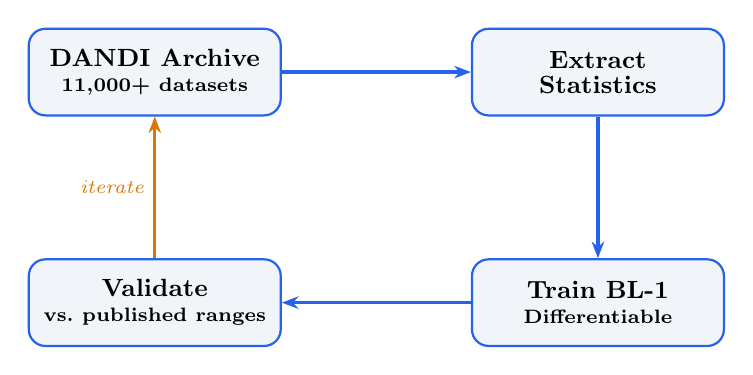
\begin{tikzpicture}[
    node distance=1.8cm and 2.4cm,
    box/.style={draw=bl1blue, fill=bl1light, rounded corners=6pt,
                minimum height=1.1cm, minimum width=3.2cm,
                font=\small\bfseries, align=center, line width=0.8pt},
    arr/.style={-{Stealth[length=6pt]}, line width=1.2pt, bl1blue},
  ]
  \node[box] (dandi)   {DANDI Archive\\[-2pt]\scriptsize 11,000+ datasets};
  \node[box, right=of dandi] (stats)  {Extract\\[-2pt]Statistics};
  \node[box, below=of stats] (train)  {Train BL-1\\[-2pt]\scriptsize Differentiable};
  \node[box, left=of train]  (validate) {Validate\\[-2pt]\scriptsize vs.\ published ranges};

  \draw[arr] (dandi)    -- (stats);
  \draw[arr] (stats)    -- (train);
  \draw[arr] (train)    -- (validate);
  \draw[arr, bl1amber] (validate) -- (dandi)
        node[midway, left, font=\scriptsize\itshape, text=bl1amber] {iterate};
\end{tikzpicture}

\vspace{10pt}
\begin{columns}[T]
\column{0.45\textwidth}
\begin{itemize}\small
  \item Load real MEA recordings (NWB)
  \item Compute firing rates, bursts, avalanches
\end{itemize}
\column{0.45\textwidth}
\begin{itemize}\small
  \item Optimise synaptic weights via gradients
  \item Validate against Wagenaar 2006 ranges
\end{itemize}
\end{columns}
\end{frame}

% --------------------------------------------------------------------------
% SLIDE 3 -- What is BL-1?
% --------------------------------------------------------------------------
\begin{frame}{What is BL-1?}
\begin{columns}[T]
\column{0.50\textwidth}
\textbf{Neuron Models}
\begin{itemize}\small
  \item Izhikevich (RS, IB, CH, FS, LTS)
  \item Adaptive Exponential (AdEx)
  \item Hybrid populations
\end{itemize}

\vspace{6pt}
\textbf{Synapses} (conductance-based)
\begin{itemize}\small
  \item AMPA \,($\tau$\,=\,2\,ms)
  \item NMDA \,($\tau$\,=\,100\,ms, Mg$^{2+}$ block)
  \item GABA\textsubscript{A} \,($\tau$\,=\,6\,ms)
  \item GABA\textsubscript{B} \,($\tau$\,=\,170\,ms)
\end{itemize}

\column{0.50\textwidth}
\textbf{Plasticity} (4 timescales)
\begin{itemize}\small
  \item Short-term (Tsodyks--Markram STP)
  \item STDP (asymmetric Hebbian)
  \item Homeostatic scaling
  \item Structural (synapse creation/pruning)
\end{itemize}

\vspace{6pt}
\textbf{Infrastructure}
\begin{itemize}\small
  \item Virtual MEA (64-ch \& 26,400 HD-MEA)
  \item Closed-loop Pong / Doom
  \item JIT-compiled via \texttt{jax.lax.scan}
  \item Differentiable (surrogate gradients)
\end{itemize}
\end{columns}
\end{frame}

% --------------------------------------------------------------------------
% SLIDE 4 -- Architecture Diagram
% --------------------------------------------------------------------------
\begin{frame}{Architecture}
\centering
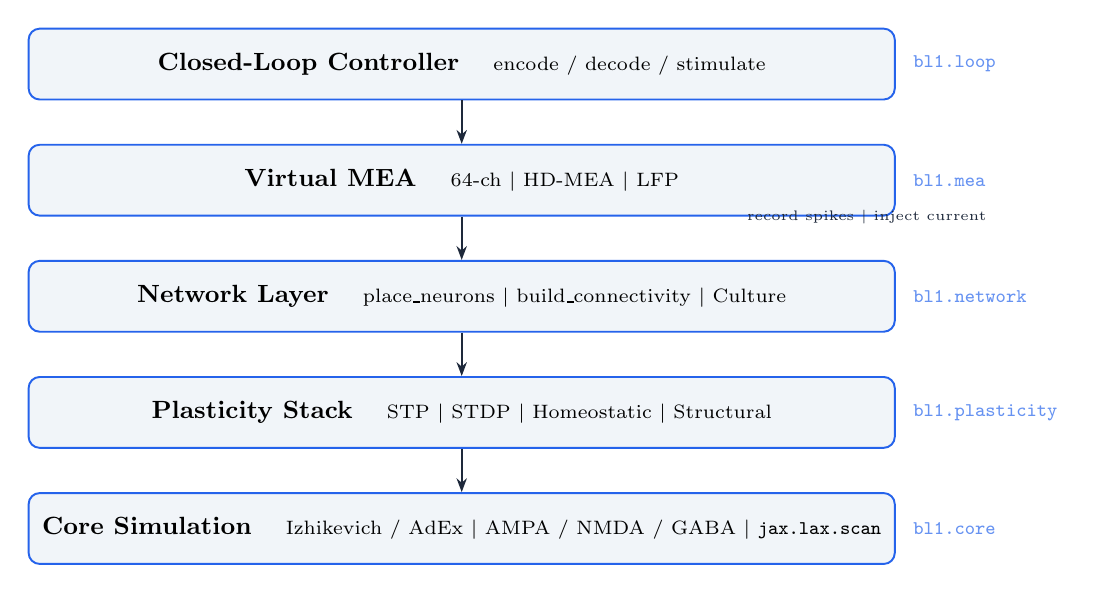
\begin{tikzpicture}[
    layer/.style={draw=bl1blue, fill=bl1light, rounded corners=4pt,
                  minimum width=11cm, minimum height=0.9cm,
                  font=\small, align=center, line width=0.7pt},
    lbl/.style={font=\scriptsize\ttfamily, text=bl1blue!70},
    arr/.style={-{Stealth[length=5pt]}, bl1dark, line width=0.6pt},
    node distance=0.55cm,
  ]
  \node[layer] (loop)  {\textbf{Closed-Loop Controller} \quad\scriptsize encode / decode / stimulate};
  \node[layer, below=of loop]  (mea)   {\textbf{Virtual MEA} \quad\scriptsize 64-ch $\vert$ HD-MEA $\vert$ LFP};
  \node[layer, below=of mea]   (net)   {\textbf{Network Layer} \quad\scriptsize place\_neurons $\vert$ build\_connectivity $\vert$ Culture};
  \node[layer, below=of net]   (plast) {\textbf{Plasticity Stack} \quad\scriptsize STP $\vert$ STDP $\vert$ Homeostatic $\vert$ Structural};
  \node[layer, below=of plast] (core)  {\textbf{Core Simulation} \quad\scriptsize Izhikevich / AdEx $\vert$ AMPA / NMDA / GABA $\vert$ \texttt{jax.lax.scan}};

  % Module labels
  \node[lbl, right=0.1cm of loop.east]  {bl1.loop};
  \node[lbl, right=0.1cm of mea.east]   {bl1.mea};
  \node[lbl, right=0.1cm of net.east]   {bl1.network};
  \node[lbl, right=0.1cm of plast.east] {bl1.plasticity};
  \node[lbl, right=0.1cm of core.east]  {bl1.core};

  % Arrows
  \draw[arr] (loop) -- (mea);
  \draw[arr] (mea) -- (net);
  \draw[arr] (net) -- (plast);
  \draw[arr] (plast) -- (core);

  % Bidirectional labels
  \node[font=\tiny, text=bl1dark, right=3.5cm of mea.south] {record spikes $\vert$ inject current};
\end{tikzpicture}
\end{frame}

% --------------------------------------------------------------------------
% SLIDE 5 -- Core Simulation Loop (Pseudocode)
% --------------------------------------------------------------------------
\begin{frame}{The Core Simulation Loop}
\begin{columns}[T]
\column{0.55\textwidth}
\begin{lstlisting}[title={\scriptsize\bfseries One timestep (JIT-compiled)}]
# Synaptic current (conductance model)
I_syn = g_ampa * (E_ampa - V)
      + g_nmda * B(V) * (E_nmda - V)
      + g_gaba * (E_gaba - V)

# Neuron update (Izhikevich)
V, u, spikes = izhikevich_step(V, u, I_syn)

# Short-term plasticity
stp_state, scale = stp_step(stp_state, spikes)

# Synapse updates
g_ampa = ampa_step(g_ampa, scale, W_exc)
g_nmda = nmda_step(g_nmda, scale, W_nmda)
g_gaba = gaba_step(g_gaba, scale, W_inh)
\end{lstlisting}

\column{0.42\textwidth}
\vspace{12pt}
\begin{block}{\small Key Design Choices}
\begin{itemize}\scriptsize
  \item Entire loop compiled via\\\texttt{jax.lax.scan} --- zero\\Python overhead
  \item Sparse connectivity via\\JAX BCOO matrices
  \item NMDA voltage-dependent\\Mg$^{2+}$ block: $B(V)$
  \item STP scale modulates\\effective synaptic weight
\end{itemize}
\end{block}

\vspace{6pt}
\centering\scriptsize\color{bl1blue}
\textbf{5.2$\times$ realtime}\\at 5K neurons on DGX Spark
\end{columns}
\end{frame}

% --------------------------------------------------------------------------
% SLIDE 6 -- DANDI Archive Integration
% --------------------------------------------------------------------------
\begin{frame}{DANDI Archive Integration}
\centering
\begin{tikzpicture}[
    step/.style={draw=bl1blue, fill=white, rounded corners=4pt,
                 minimum height=0.9cm, minimum width=2.7cm,
                 font=\scriptsize, align=center, line width=0.7pt},
    arr/.style={-{Stealth[length=5pt]}, bl1blue, line width=1pt},
    node distance=0.4cm and 0.6cm,
  ]
  \node[step] (browse) {Browse DANDI\\catalog};
  \node[step, right=of browse] (download) {Download NWB\\recordings};
  \node[step, right=of download] (load) {\texttt{load\_nwb\_spike\_trains}\\(bl1.validation.loaders)};
  \node[step, right=of load] (raster) {Spike trains\\$\to$ raster};
  \node[step, right=of raster] (stats) {Compute\\statistics};

  \draw[arr] (browse) -- (download);
  \draw[arr] (download) -- (load);
  \draw[arr] (load) -- (raster);
  \draw[arr] (raster) -- (stats);
\end{tikzpicture}

\vspace{14pt}
\begin{columns}[T]
\column{0.30\textwidth}
\centering\small\textbf{Rat Cortical HD-MEA}\\
\scriptsize DANDI 001611\\2,700 NWB files, 39.9\,GB\\
950 channels, repeated stim

\column{0.30\textwidth}
\centering\small\textbf{DishBrain}\\
\scriptsize OSF 5u6qv\\
Closed-loop Pong\\
Mouse + human iPSC

\column{0.30\textwidth}
\centering\small\textbf{Organoid HD-MEA}\\
\scriptsize Zenodo 6578989\\
40 files, 70.9\,GB\\
Human brain organoid slices
\end{columns}

\vspace{10pt}
{\small Also catalogued: Wagenaar 2006, Beggs \& Plenz 2003, Kapucu 2022,
Heiney 2022, van der Molen 2025, Braingeneers SpikeCanvas (\textbf{11 datasets total})}
\end{frame}

% --------------------------------------------------------------------------
% SLIDE 7 -- Differentiable Training Loop
% --------------------------------------------------------------------------
\begin{frame}{Differentiable Training: The Key Innovation}
\begin{columns}[T]
\column{0.58\textwidth}
\begin{lstlisting}[title={\scriptsize\bfseries Training loop (pseudocode)}]
# 1. Load real recording from DANDI
real_stats = load_and_analyze(nwb_file)

# 2. Initialise BL-1 culture
W_exc, W_inh = init_weights(n_neurons=5000)

for epoch in range(N_epochs):
    # Forward pass (fully differentiable)
    spikes = simulate(W_exc, W_inh, I_noise)
    sim_stats = compute_statistics(spikes)

    # Loss: match real data
    loss = (sim_stats.fr - real_stats.fr)**2
         + (sim_stats.burst - real_stats.burst)**2
         + synchrony_loss(spikes)
         + weight_reg(W_exc, W_inh)

    # Backward pass (surrogate gradients)
    grads = jax.grad(loss)(W_exc, W_inh)
    W_exc, W_inh = adam.update(grads)
\end{lstlisting}

\column{0.39\textwidth}
\vspace{8pt}
\begin{block}{\small How It Works}
\begin{itemize}\scriptsize
  \item Spike non-differentiability solved\\by \textbf{SuperSpike} surrogate:\\
        $\sigma'(V) \approx \frac{\beta}{(1 + \beta|V-V_{\mathrm{th}}|)^2}$
  \item Gradients flow through the\\
        \textbf{entire simulation}:\\
        synapses $\to$ neurons $\to$ spikes\\
        $\to$ statistics $\to$ loss
  \item Optimiser: Adam (optax)
  \item Dale's law \& sparsity\\preserved throughout
\end{itemize}
\end{block}

\vspace{6pt}
\centering

\begin{tikzpicture}
  \node[draw=bl1green, fill=bl1green!10, rounded corners=3pt,
        font=\scriptsize\bfseries, text=bl1green, inner sep=4pt]
    {Fit to ANY recording};
\end{tikzpicture}
\end{columns}
\end{frame}

% --------------------------------------------------------------------------
% SLIDE 8 -- Biological Validation Results
% --------------------------------------------------------------------------
\begin{frame}{Biological Validation: Wagenaar 2006}
\centering
\small
\begin{tabular}{lrrrc}
\toprule
\textbf{Metric} & \textbf{BL-1 Sim} & \multicolumn{2}{c}{\textbf{Published Range}} & \textbf{Status} \\
\midrule
Firing rate (Hz)       & 1.6        & 0.1   & -- 5.0    & \textcolor{bl1green}{\textbf{PASS}} \\
Burst rate (/min)      & 6--11      & 0.2   & -- 20     & \textcolor{bl1green}{\textbf{PASS}} \\
Burst duration (ms)    & 95--116    & 100   & -- 2000   & \textcolor{bl1green}{\textbf{PASS}} \\
IBI mean (s)           & 4.5--10.3  & 3     & -- 300    & \textcolor{bl1green}{\textbf{PASS}} \\
IBI CV                 & 0.45--1.15 & 0.3   & -- 2.0    & \textcolor{bl1green}{\textbf{PASS}} \\
Recruitment            & 48--67\%   & 10    & -- 95\%   & \textcolor{bl1green}{\textbf{PASS}} \\
\bottomrule
\end{tabular}

\vspace{12pt}

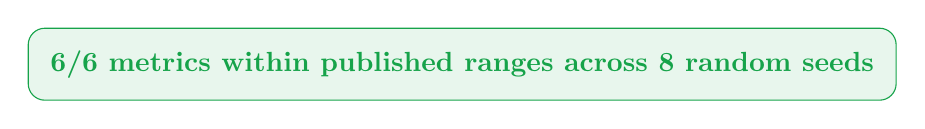
\begin{tikzpicture}
\node[draw=bl1green, fill=bl1green!10, rounded corners=6pt,
      font=\bfseries, text=bl1green, inner sep=8pt]
  {6/6 metrics within published ranges across 8 random seeds};
\end{tikzpicture}

\vspace{8pt}
\scriptsize
5,000 neurons $\cdot$ 60\,s simulation $\cdot$ AMPA/NMDA split (37\% NMDA) $\cdot$ STP depression ($U$\,=\,0.30, $\tau_{\mathrm{rec}}$\,=\,800\,ms)
\end{frame}

% --------------------------------------------------------------------------
% SLIDE 9 -- GPU Performance
% --------------------------------------------------------------------------
\begin{frame}{GPU Performance}
\centering
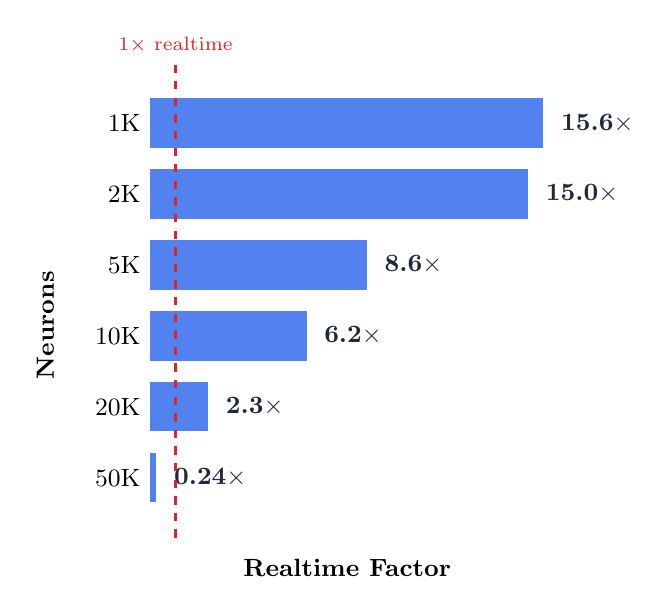
\begin{tikzpicture}
  \pgfmathsetmacro{\bw}{0.9}
  \pgfmathsetmacro{\scale}{0.32}
  % Data: neurons, RT factor
  \foreach \n/\rt/\y [count=\i] in {
    1K/15.6/6, 2K/15.0/5, 5K/8.6/4, 10K/6.2/3, 20K/2.3/2, 50K/0.24/1
  }{
    % Bar
    \fill[bl1blue!80] (0, \y*\bw) rectangle (\rt*\scale, \y*\bw+\bw*0.7);
    % Label left
    \node[left, font=\small] at (0, \y*\bw+\bw*0.35) {\n};
    % Value right
    \node[right, font=\small\bfseries, text=bl1dark] at (\rt*\scale+0.1, \y*\bw+\bw*0.35) {\rt$\times$};
  }
  % Realtime line
  \draw[dashed, bl1red, line width=0.8pt] (1*\scale, 0.5*\bw) -- (1*\scale, 7.2*\bw)
    node[above, font=\scriptsize, text=bl1red] {1$\times$ realtime};
  % Axis labels
  \node[below, font=\small\bfseries] at (2.5, 0.3) {Realtime Factor};
  \node[left, font=\small\bfseries, rotate=90, anchor=south] at (-1.1, 3.5*\bw) {Neurons};
\end{tikzpicture}

\vspace{8pt}
\small
NVIDIA DGX Spark (GB10) $\cdot$ JAX 0.9.2 $\cdot$ CUDA 13 $\cdot$ 5\,s simulated per benchmark
\end{frame}

% --------------------------------------------------------------------------
% SLIDE 10 -- What's Next
% --------------------------------------------------------------------------
\begin{frame}{What's Next}
\begin{columns}[T]
\column{0.50\textwidth}
\textbf{Near-term}
\begin{itemize}\small
  \item Fit to individual DANDI recordings\\
        {\scriptsize per-culture weight optimisation}
  \item DishBrain replication\\
        {\scriptsize closed-loop Pong with FEP feedback}
  \item Pharmacology validation\\
        {\scriptsize TTX, CNQX, Bicuculline dose--response}
\end{itemize}

\column{0.50\textwidth}
\textbf{Longer-term}
\begin{itemize}\small
  \item Morphological neurons (Jaxley)\\
        {\scriptsize compartmental models on GPU}
  \item Organoid simulations\\
        {\scriptsize 3D cultures, layered connectivity}
  \item Community validation\\
        {\scriptsize 11 catalogued datasets, ModelDB lineage}
  \item ViZDoom 3D environments\\
        {\scriptsize beyond Pong}
\end{itemize}
\end{columns}

\vspace{16pt}
\centering

\begin{tikzpicture}
\node[draw=bl1blue, fill=bl1blue!10, rounded corners=6pt,
      font=\small, inner sep=10pt, text width=12cm, align=center]
  {\textbf{Open source} $\cdot$ MIT licence $\cdot$ \texttt{github.com/m9h/bl1}\\[2pt]
   JAX $\cdot$ GPU-ready $\cdot$ Differentiable $\cdot$ Validated};
\end{tikzpicture}
\end{frame}

\end{document}
